\documentclass[UTF8,a4paper]{ctexart}
\usepackage{geometry} % 设置页边距,页面大小
\geometry{left=2.5cm,right=2.0cm,top=2.50cm,bottom=2.0cm}
\linespread{1.3}%调整行间距
\usepackage{graphicx} % 引入图片
%\usepackage[justification=centering]{caption} % 图片的caption居中
\usepackage[indent]{caption} % 设置图片的 caption 换行缩进

\pagestyle{plain}    
\usepackage{setspace} %行间距
\usepackage{array} %
\usepackage{booktabs} %调整表格线与上下内容的间隔
\usepackage{multirow}
\usepackage{hyperref} %加入书签跳转
\usepackage{fontspec} %引入字体Times New Roman字体
%\setmainfont{Times New Roman}             %设置正文字体为Times New Roman
\usepackage{abstract} % 修改摘要

%\usepackage[fontset=windows]{ctex}
\usepackage{xeCJK} %调用系统中已安装的字体
\setCJKmainfont{SimSun}
\setmainfont{Times New Roman}
%% 支持汉字加粗
\let\heiti\relax % 黑体
\newCJKfontfamily\heiti{SimHei}[AutoFakeBold]
\setCJKsansfont{SimHei}[AutoFakeBold]

\let\songti\relax % 宋体
\newCJKfontfamily\songti{SimSun}[AutoFakeBold]
\setCJKmainfont{SimSun}[AutoFakeBold]  



%% 目录格式设置
\usepackage{tocloft}      %必须这么写,否则会报错
\renewcommand{\contentsname}{\centerline{\Large{\heiti{目\quad\quad 录}}}}
%\renewcommand{\cftchapleader}{\cftdotfill{0.6}} %设置chapter条目的引导点间距
\renewcommand{\cftsecleader}{\cftdotfill{0.6}}
\renewcommand{\cftsubsecleader}{\cftdotfill{0.6}}
\renewcommand{\cftsubsubsecleader}{\cftdotfill{0.6}}
%\renewcommand{\cftchapfont}{\hts}    %设置chapter条目的字体
\renewcommand{\cftsecfont}{\heiti}    %设置section条目的字体
\renewcommand{\cftsecfont}{\Large}    %设置section条目的四号
\renewcommand{\cftsubsecfont}{\songti} %设置subsection条目的字体
\renewcommand{\cftsubsecfont}{\large} %设置subsection条目的字体
\renewcommand{\cftsubsubsecfont}{\songti} %设置subsection条目的字体
\renewcommand{\cftsubsubsecfont}{\large} %设置subsection条目的字体


% 数学公式
\usepackage{amsmath}

% 插入代码块
\usepackage{listings}
\usepackage{xcolor}
\lstset{
 %language=bash,                % the language of the code
 columns=fixed,       
% numbers=left,                                        % 在左侧显示行号
% numberstyle=\tiny\color{gray},                       % 设定行号格式
 frame=none,                                          % 不显示背景边框
 backgroundcolor=\color[RGB]{245,245,244},            % 设定背景颜色
 keywordstyle=\color[RGB]{40,40,255},                 % 设定关键字颜色
 numberstyle=\footnotesize\color{darkgray},           
 commentstyle=\it\color[RGB]{0,96,96},                % 设置代码注释的格式
% stringstyle=\rmfamily\slshape\color[RGB]{128,0,0},   % 设置字符串格式
}


% 参考文献
\usepackage{cite}
%%%%%%%%%%%%%%%%%%%%%%%%%%%%%%%%%%%%%%%%%%%%%%%%%%%%%%%%%%%%%%%%%%%%%%%%%%%%%%%%%
%  以下是论文内容
%%%%%%%%%%%%%%%%%%%%%%%%%%%%%%%%%%%%%%%%%%%%%%%%%%%%%%%%%%%%%%%%%%%%%%%%%%%%%%%%%
%  正文
\begin{document}
%% 封面
% 这是封面
\begin{flushright}
\end{flushright}
\begin{center}
    \vskip 1.5cm
    
\includegraphics[scale=0.6]{figs/ncepu.eps}%学校图标
\end{center}
\begin{center}
    \vskip 1.5cm
    
\includegraphics[scale=0.6]{figs/bthesistitle.eps}%毕业设计图标
\end{center}
\begin{center}
  \vskip 2cm
    \fontsize{15}{1} \textbf{题目} \underline{基于Qemu模拟器移植rCore操作系统的开发与实现}
  \vskip 2.5cm
\end{center}
\begin{center}
  \begin{tabular}{l}

    院\quad\quad 系 \underline{\qquad 控制与计算机工程学院 \quad }\\\\
    专\quad\quad 业 \underline{\qquad 计算机科学与技术 \quad\qquad}\\\\
    % \quad 代表空格,输入题目后自己调长度
    班\quad\quad 级 \underline{\qquad\quad 计算1702班 \quad\qquad\quad }\\\\
    学生姓名 \underline{\qquad\qquad 杨秉学\qquad\qquad\qquad}\\\\
    学\quad\quad 号 \underline{\qquad\quad 120171080212 \qquad\qquad }\\\\
    指导教师 \underline{\qquad\qquad\quad 琚贇\qquad\qquad\qquad }\\\\

  \end{tabular}
\end{center}
\begin{center}
        \vskip 2.5cm
    {2021} 年{\quad 六\quad }月{\qquad \qquad }日

\end{center}
\thispagestyle{empty} %去除本页页码
      
%%摘要
%%%% 中文摘要
% 这是中文摘要
\newpage
\pagenumbering{Roman}
\renewcommand{\abstractname}{\heiti{\Large{摘\quad \quad \quad \quad 要}}}
\begin{abstract}
\addcontentsline{toc}{section}{\heiti{\Large{摘 \quad \quad 要}}}    
{\large{本实验是验证性实验,将Linux移植到RiSC-V的平台,可以实现完成基本功能,并借此机会回顾本科所学的全部内容}}

%\\ \hspace*{\fill} \\  %换行,用空格填充,再换行,即可实现空出一整行的效果,不需任何环境调整
\noindent %取消首航缩进
    {\large{\textbf{关键字}:RISC-V,Qemu,linux}}
\end{abstract}

%%%% 英文摘要
% 这是英文摘要
\newpage
\renewcommand{\abstractname}{\Large \textbf{ABSTRACT}}
\begin{abstract}
\addcontentsline{toc}{section}{\heiti{\Large{ABSTRACT}}}    
{\large{This experiment is a confirmative experiment. By porting Linux to RISC-V platform, the basic functions can be realized. And this opportunity is used to review all the contents learned in the undergraduate course}}

\noindent
\textbf{KEY WORDS:}RISC-V,Qemu,linux
\end{abstract}

%% 目录
\newpage
\tableofcontents
\thispagestyle{empty}

%% 章节
\newpage
\pagenumbering{arabic}
%%%%定制标题样式
%%%%% section
\CTEXsetup[name={第,章 },format={\centering\heiti\zihao{-2}},aftername={\enspace},beforeskip={24bp},afterskip={18bp}]{section} %name选项中不要使用中文逗号 \zihao(-2)字号小二
%%%%% subsection
\CTEXsetup[format={\raggedright\songti\zihao{-3}},aftername={\enspace},beforeskip={24bp},afterskip={6bp}]{subsection}
%%%%% subsubsection
\CTEXsetup[format={\raggedright\songti\zihao{4}},aftername={\enspace},beforeskip={12bp},afterskip={6bp}]{subsubsection}

% 本章节是介绍项目的背景信息
\section{绪论}
\subsection{课题研究背景和意义}
在“中兴事件”刚过没多久,某国家就开始发起“华为事件”,进行各种制裁,对我国半导体产业的打击极大,放眼整个产业链,我们国家连一个像样的指令集架构都没有,当我们想研究开发产品竟然还需要别人来授权,这是莫大的耻辱。为什么别人能做出来,我们就做不出来,我们也并不比他们差什么。所以,我觉得我有必要研究这样的问题了,这就是我大学为什么在其他人都要研究人工智能这些内容的时候,我偏偏要研究这些偏底层的原理。

Risc-v是一个最近流行基于RISC指令集架构,类似与软件领域开源的linux一样,Risc-V也有很多领域可以发挥作用,如果将linux与RiSC-V结合一起来发展的话,我们国家可以利用已有的成就上完成自己的目标,而且开源的话可以大家一起参与进来,在这个过程中可以发现自己的不足,然后改正。


\subsection{国内外研究现状}
首先RISC-V是由国外的Berkeley大学开发的,我们承认与其之间存在差距,但是这都无所谓,就算他们现在比我们发展要靠前但这不代表永远都比我们要靠前,如果我们把精力,资源放在这方面,假以时日我们是会迎头赶上的,也可以做出属于自己的产业链。

目前国外SiFive公司做的不错,国内的芯来科技模仿SiFive做的也不错,阿里也有自己的研究。

\subsection{本文研究内容}
虽然,已经国内已经有人做出了基于RISC-V处理器内核,linus也把riscv-linux合并到Linux的主分支上了,但是我在这个毕设的内容就是自己进行一遍,是验证性的实验,虽然我也知道我做的这些东西微不足道,但是我想既然我开始做了,应该是会往好的方向发展的。

在过程中复习了一下本科所学得全部知识,这为我日后的发展打下了坚实的基础。


\newpage  % 课题研究背景和意义
% 本章节是介绍实验流程
\section{相关工作}
本实验是参考Github上的项目 \cite{BusyBear} 来实现的,但是当时的很多内容已经不适用了,比方说当时采用Linux Kernel v4.4当时Linux主分支不支持RISC-V,但是这里采用的是Linux Kernel v5.*,此时Linux主分支已经支持了RISC-V架构了;还有就是Qemu在4.*的时候需要自己编译 OpenSBI ,但是在Qemu 5.*以后就内嵌 OpenSBI,一些流程也有所改变,但是清楚Linux启动流程就可以了,详细参考\cite{从按下电源开始的一场接力赛}。

\subsection{实验平台}
本实验环境是在Intel的 x86 平台,运行系统是Gentoo linux的,系统具体信息如图\ref{fig:gentoo} 所示,实验所需的软件信息如图\ref{fig:info}。

\begin{figure}[htbp]
  \centering %居中显示
  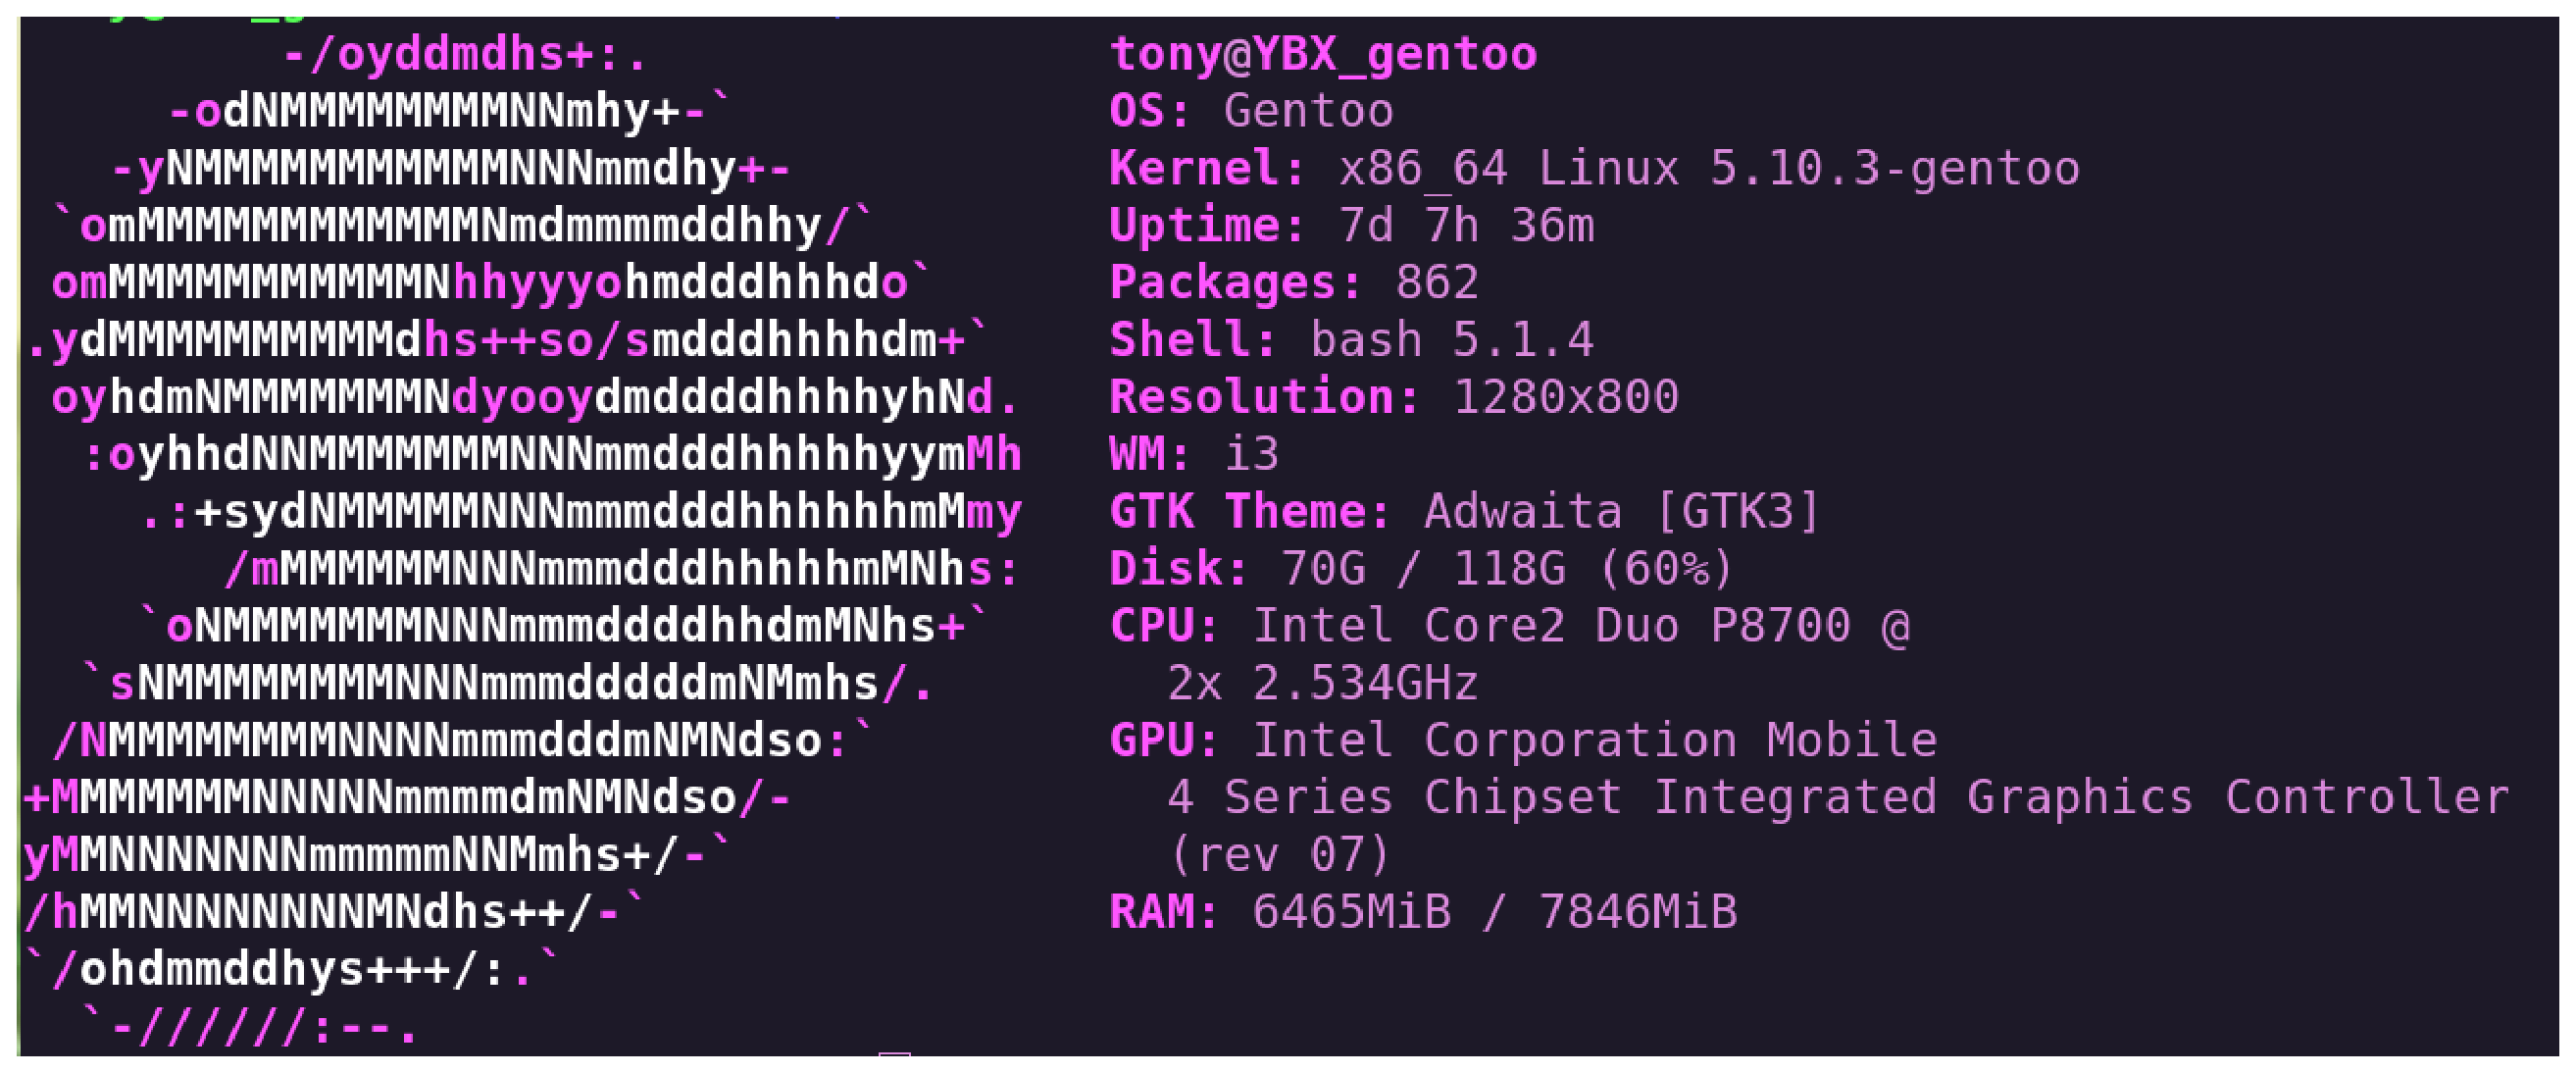
\includegraphics[width=0.8 \textwidth]{figs/Process/gentoo_Logo.eps}
  \caption{实验操作系统}
  \label{fig:gentoo} %设置图形引用名称
\end{figure}

\begin{figure}[htbp]
  \centering %居中显示
  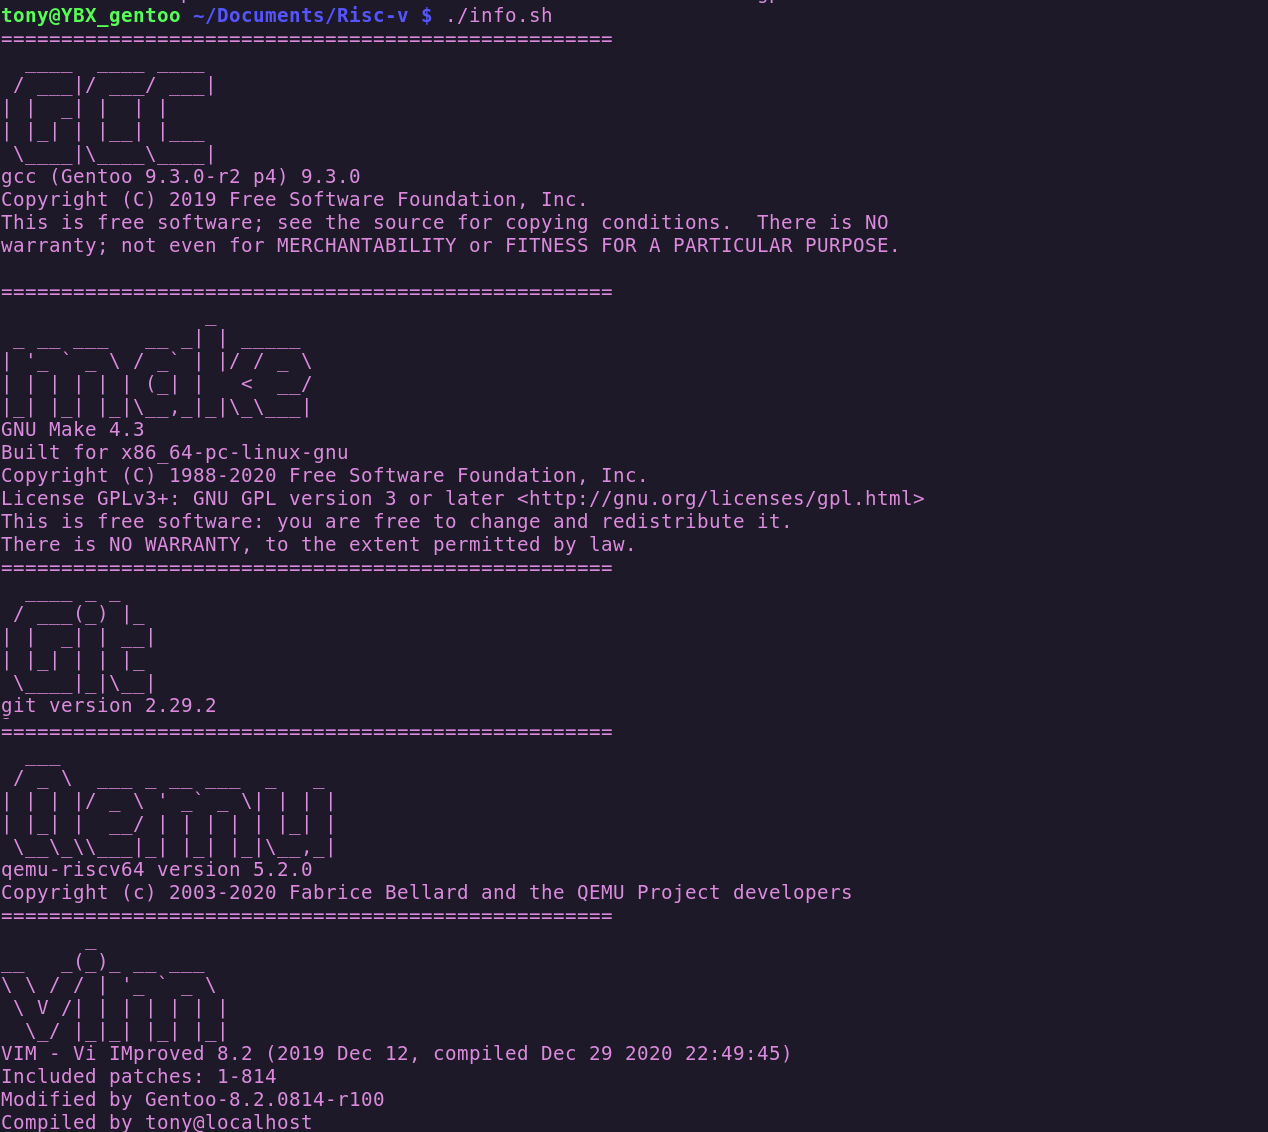
\includegraphics[width=1.0 \textwidth]{figs/Process/info.png}
  \caption{实验所需软件信息}
  \label{fig:info} %设置图形引用名称
\end{figure}

\subsection{Qemu搭建}
在 Gentoo 官方的 Wiki 手册中可以参考 \cite{GentooQemu}
\subsubsection{检测处理器是否支持虚拟化}
\begin{lstlisting}
\$ grep --color -E "vmx|svm" /proc/cpuinfo 
\end{lstlisting}
如果能显示出 图\ref{fig:vmx_svm} 说明处理器是支持虚拟化的

\begin{figure}[htbp]
  \centering %居中显示
  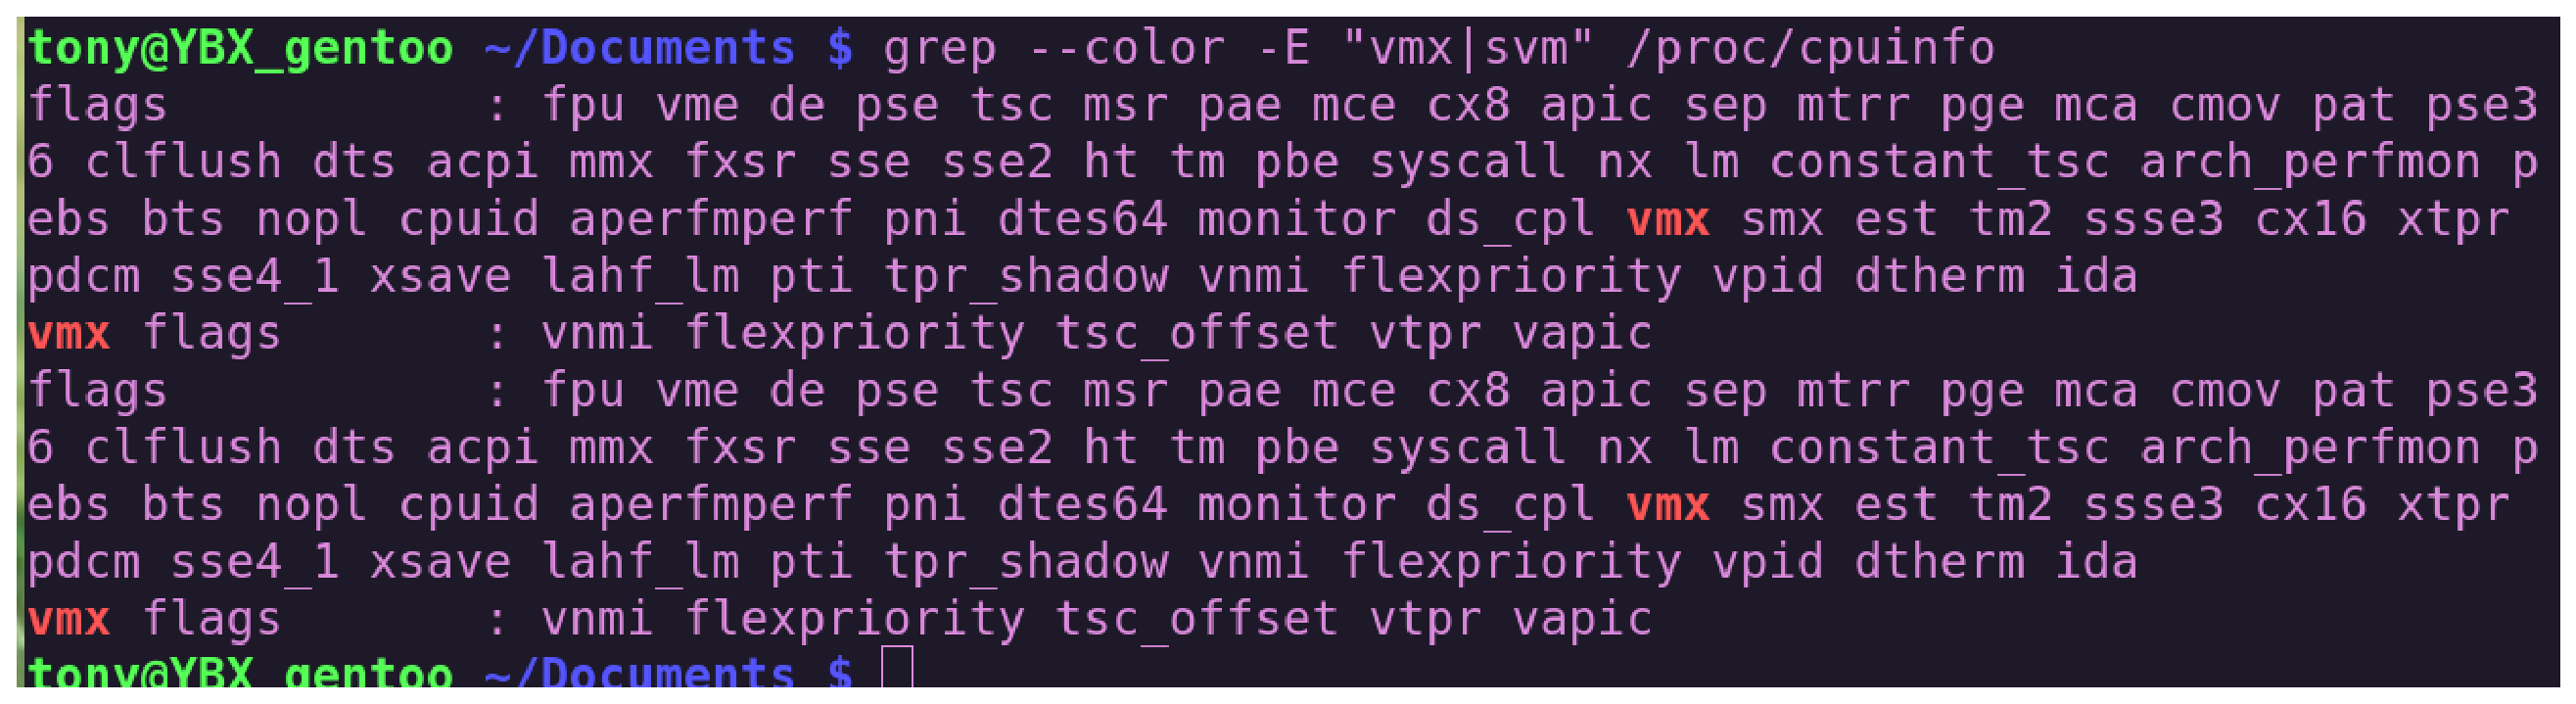
\includegraphics[width=0.8 \textwidth]{figs/Process/vmx_svm.eps}
  \caption{是否支持虚拟化}
  \label{fig:vmx_svm} %设置图形引用名称
\end{figure}

\subsubsection{编译内核}
首先需要更改内核配置

\begin{lstlisting}
cd /usr/src/linux
make menuconfig 
\end{lstlisting}

然后根据以下步骤进行配置内核,使其支持KVM,其中 图\ref{fig:KVM_Intel} 是根据自己处理器来选择的,我的是Intel的处理器,如果使用AMD处理器的话,需要勾选另一个。

\begin{figure}[htbp]
  \centering %居中显示
  \includegraphics[width=0.9 \textwidth]{figs/Process/Kernel/Step1.eps}
  \caption{Virtualization}
  \label{fig:Virtualization} %设置图形引用名称
\end{figure}

\begin{figure}[htbp]
  \centering %居中显示
  \includegraphics[width=0.9 \textwidth]{figs/Process/Kernel/Step2.eps}
  \caption{Kernel-based Virtual Machine (KVM) support}
  \label{fig:Kernel-based} %设置图形引用名称
\end{figure}

\begin{figure}[htbp]
  \centering %居中显示
  \includegraphics[width=0.9 \textwidth]{figs/Process/Kernel/Step3.eps}
  \caption{KVM for Intel processors support}
  \label{fig:KVM_Intel} %设置图形引用名称
\end{figure}

\subsubsection{修改USE Flags并安装}
\begin{lstlisting}
# vim /etc/portage/make.conf
QEMU_SOFTMMU_TARGETS="riscv32 risc64"
QEMU_USER_TARGETS="x86_64"

# vim /etc/portage/package.use
app-emulation/qemu qemu_softmmu_targets_arm qemu_softmmu_targets_x86_64 
                 qemu_softmmu_targets_sparc
app-emulation/qemu qemu_user_targets_x86_64

% 进行安装
# emerge --ask app-emulation/qemu -y
\end{lstlisting}

\subsection{简便方法}
这个步骤是比较偷懒的方式,你可以直接下载网上已经提供编译好而且运行没问题的二进制包,直接运行,但是我下载了,就没运行成功,所以就没有截图演示。
\begin{lstlisting}
cd release
wget -c \ 
> https://github.com/michaeljclark/busybear-linux/releases/download/v1.0/
  bbl.bz2

wget -c \
> https://github.com/michaeljclark/busybear-linux/releases/download/v1.0/
  busybear.bin.bz2

bzip2 -d *.bz2
\end{lstlisting}

\subsection{安装GNU工具链}

\begin{lstlisting}
mkdir YBX-bishe
cd YBX-bishe/
# 拉取 gnu-toolchain
git clone --recursive https://github.com/riscv/riscv-gnu-toolchain

# 编译生成 RISC-V newlib & Linux toolchains
cd riscv-gnu-toolchain
./configure --prefix=/opt/riscv --enable-multilib
make newlib -j5
make linux -j5
export PATH=$PATH:/opt/riscv/bin
export RISCV=/opt/risc
$
\end{lstlisting}

\subsection{创建根文件系统}
\begin{lstlisting}
cd ..
git clone https://github.com/michaeljclark/busybear-linux.git
cd busybear-linux
make -j5
\end{lstlisting}

但是这没完,因为busybear会自动帮你下载好 busybox 但是需要自己进行解压和编译

\begin{lstlisting}
CROSS_COMPILE=riscv{{bits}}-unknown-linux-gnu- make menuconfig
CROSS_COMPILE=riscv{{bits}}-unknown-linux-gnu- make
\end{lstlisting}

下面咱们就要制做最小文件系统
\begin{lstlisting}
qemu-img create rootfs.img  1g
mkfs.ext4 rootfs.img
mkdir rootfs
sudo mount -o loop rootfs.img  rootfs
cd rootfs
sudo cp -r ../busyboxsource/_install/* .
sudo mkdir proc sys dev etc etc/init.d
cd etc/init.d/
sudo touch rcS
sudo vi rcS
#!/bin/sh
mount -t proc none /proc
mount -t sysfs none /sys
/sbin/mdev -s

sudo mod +x rcS
sudo umount rootfs
\end{lstlisting}

\subsection{构建Linux内核}
\begin{lstlisting}
git clone https://github.com/torvalds/linux
cd linux
git checkout v5.4
make ARCH=riscv CROSS_COMPILE=riscv64-unknown-linux-gnu- defconfig
make ARCH=riscv CROSS_COMPILE=riscv64-unknown-linux-gnu-
\end{lstlisting}

\subsection{制作BootLoader——BBL(Berkeley Boot Loader)}
其实在完成这一步之前需要先链接一下计算机启动的过程需要经历哪几步,由《从按下电源开始的一场接力赛》\cite{从按下电源开始的一场接力赛},简单概括一下Linux的开机流程如图\ref{fig:Linux_boot},大致5步。首先经过BIOS/UEFI自检,然后是MBR,接着是OBR,然后轮到Boot Loader,最后是OS的自举

\begin{figure}[htbp]
  \centering %居中显示
  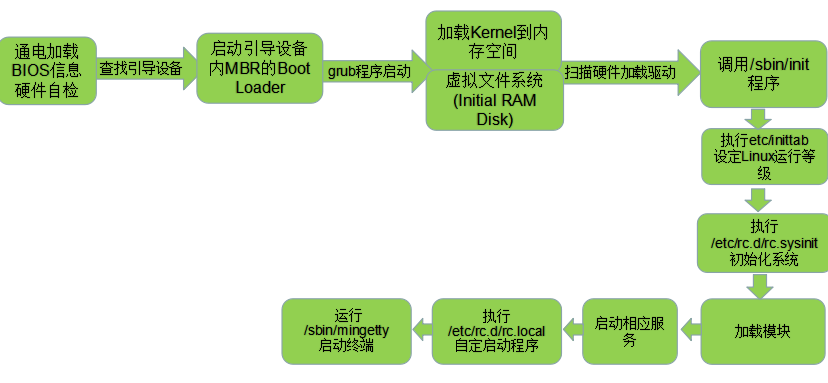
\includegraphics[width=0.9 \textwidth]{figs/Process/Linux开机流程.png}
  \caption{Linux开机流程}
  \label{fig:Linux_boot} %设置图形引用名称
\end{figure}

\begin{lstlisting}
cd..
git clone https://github.com/riscv/riscv-pk.git
cd riscv-pk
mkdir build
cd build
../configure \
> --enable-logo \
> --host=riscv64-unknown-elf \
> --with-payload=../../riscv-linux/vmlinux

make -j8
\end{lstlisting}

\subsection{编写各种所需脚本}
\begin{lstlisting}
cd ..
mkdir Running
cd Running
\end{lstlisting}
创建KVM启动脚本
\begin{lstlisting}
vim open_kvm
#!/bin/sh
sudo /etc/init.d/libvirtd start
sudo virsh net-start default  #开启网络服务
\end{lstlisting}

创建KVM关闭脚本
\begin{lstlisting}
sudo virsh net-destory default
sudo /etc/init.d/libvirtd stop
\end{lstlisting}


创建网络启动脚本
\begin{lstlisting}
#!/bin/sh
brctl addif virbr0 $1
ifconfig $1 up
\end{lstlisting}

创建网络关闭脚本
\begin{lstlisting}
#!/bin/sh
ifconfig $1 down
brctl delif virbr0 $1
\end{lstlisting}

创建程序运行脚本
\begin{lstlisting}
#!/bin/sh
# QEMU 5.2以后.模拟器内部集成了OpenSBI
sudo qemu-system-riscv64 \
  -nographic -machine virt \
  -m 1024M \
  -kernel bbl \
  -kernel ~/Documents/Risc-v/busybear-linux/build/linux-5.0/arch
                  /riscv/boot/Image \
  -drive file=busybear.bin,format=raw,id=hd0 \
  -device virtio-blk-device,drive=hd0 \
  -device virtio-net-device,netdev=net0 \
  -netdev type=tap,script=./ifup.sh,downscript=./ifdown.sh,id=net0 \
  -append "root=/dev/vda ro console=ttyS0" 
\end{lstlisting}

\subsection{运行}
\begin{lstlisting}
./Running.sh
\end{lstlisting}

\subsection{最终效果}
最终结果如图\ref{fig:success},具体实验流程视频演示可以看 \cite{结果演示},里面记录种种失败经历和解决方案。
\begin{figure}[htbp]
  \centering %居中显示
  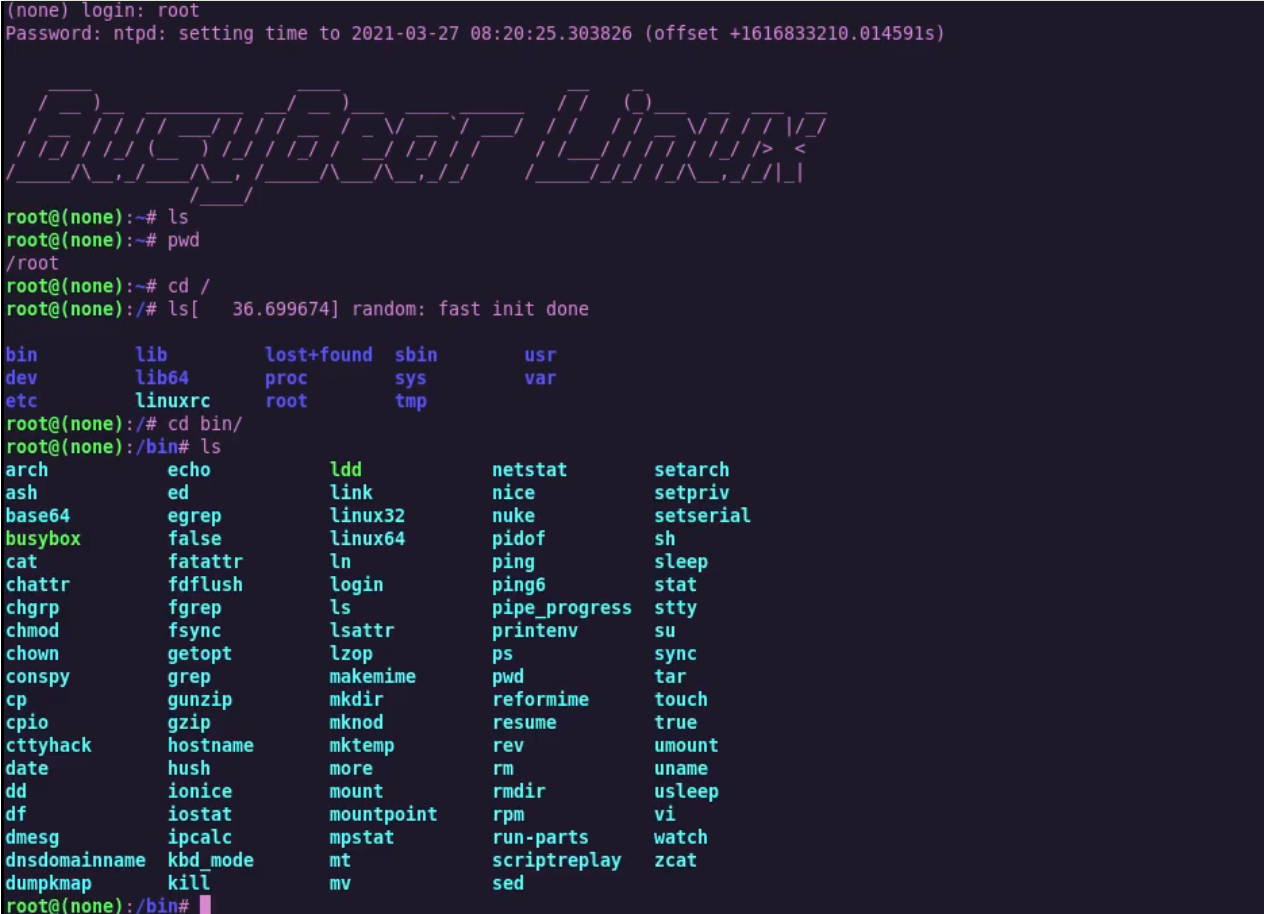
\includegraphics[width=0.9 \textwidth]{figs/Process/success.png}
  \caption{运行成功}
  \label{fig:success} %设置图形引用名称
\end{figure}








\newpage % 相关工作
% 本章节介绍RISC-V的原理
\section{Risc-V模拟器原理}
\subsection{KVM \& Qemu}
首先Qemu(Quick Emulator)本身并不完全是KVM的一部分,它是一套由软件模拟实现的。

而KVM(Kernel Virtual Machine)是有两部分组成,一部分是Linux内核的KVM模块,另一块是经过简化后的Qemu。它能够让Linux主机成为一个Hypervisor(虚拟机监控器)。在支持VMX(Virtual    Machine Extension)功能的x86处理器中,Linux在原有的用户模式和内核模式中新增加了客户模式,并且客户模式也拥有自己的内核模式和用户模式,虚拟机就是运行在客户模式中。三层结构如   图\ref{fig:kvm}

\begin{figure}[htbp]
  \centering %居中显示
  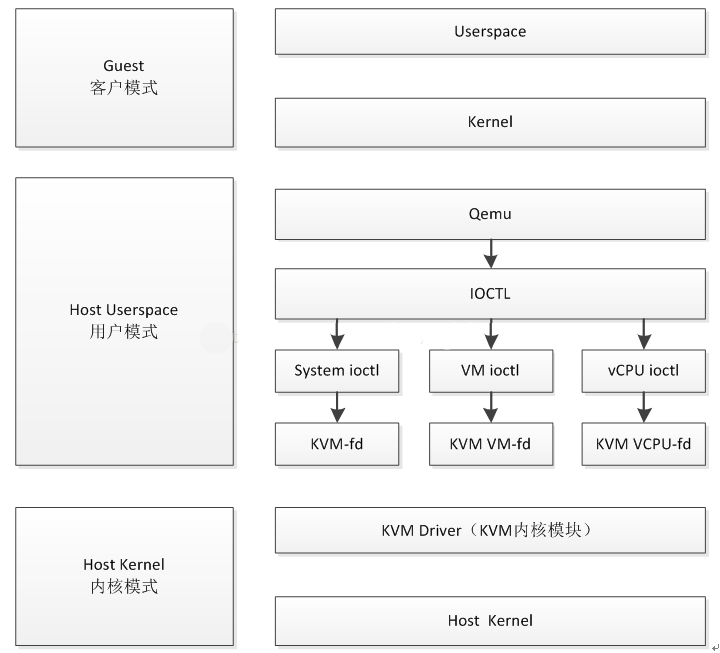
\includegraphics[width=0.7 \textwidth]{figs/KVM三种模式的层次关系.png}
  \caption{KVM三种模式的层次关系}
  \label{fig:kvm} %设置图形引用名称
\end{figure}
%『h』当前位置。将图形放置在正文文本中给出该图形环境的地方。如果本页所剩的页面不够,这一参数将不起作用。
%『t』顶部。将图形放置在页面的顶部。
%『b』底部。将图形放置在页面的底部。
%『p』浮动页。将图形放置在一只允许有浮动对象的页面上。










\newpage %介绍RISC-V模拟器的原理
% 性能评估
% 本章节介绍与前人的比较
\section{与前人比较}
本实验是参考Github上的项目 \cite{BusyBear} 实现的,但是在实验工程已经三年多没有更新,其中很多功能已经失效了,根据README.md文件很多步骤会报错,可详见实验结果\cite{结果演示},但是最后都想办法解决。
通过该实验,我对Qemu有更深的理解,再加上对操作系统底层有更深的理解,更深体会到编译工具的熟练使用。



\newpage  %与前人比较


%% 参考文献
\bibliographystyle{plain}
\bibliography{Ref}
%\bibliographystyle{plain}指定参考文献的呈现方式,常见的预设样式的可选项有8种,分别是:
%% 1. plain,按字母的顺序排列,比较次序为作者、年度和标题;
%% 2. unsrt,样式同plain,只是按照引用的先后排序;
%% 3. alpha,用作者名首字母+年份后两位作标号,以字母顺序排序;
%% 4. abbrv,类似plain,将月份全拼改为缩写,更显紧凑;
%% 5. ieeetr,国际电气电子工程师协会期刊样式;
%% 6. acm,美国计算机学会期刊样式;
%% 7. siam,美国工业和应用数学学会期刊样式;
%% 8. apalike,美国心理学学会期刊样式;
\end{document}
